\documentclass[11pt]{article}
\usepackage[textwidth=18.0cm, textheight=23.0cm, top=2.0cm]{geometry}
\usepackage{pst-all}
\usepackage{amssymb}
\usepackage{tikz}
\usepackage{underscore}\begin{document}
\pagestyle{empty}


ClassName: \underline{\textbf{Class_03.2bp-26}}
\par
BinSize: \underline{\textbf{40 × 40}}
\par
ReduceSize: \underline{\textbf{40 × 40}}
\par
TypeNum: \underline{\textbf{59}}
\par
Num: \underline{\textbf{60}}
\par
OutS: \underline{\textbf{17600}}
\par
InS: \underline{\textbf{15937}}
\par
Rate: \underline{\textbf{0.906}}
\par
UB: \underline{\textbf{11}}
\par
LB0: \underline{\textbf{11}}
\par
LB: \underline{\textbf{11}}
\par
LBWithCut: \underline{\textbf{11}}
\par
NodeCut: \underline{\textbf{0}}
\par
ExtendedNodeCnt: \underline{\textbf{1}}
\par
GenNodeCnt: \underline{\textbf{1}}
\par
PrimalNode: \underline{\textbf{0}}
\par
ColumnCount: \underline{\textbf{11}}
\par
TotalCutCount: \underline{\textbf{0}}
\par
RootCutCount: \underline{\textbf{0}}
\par
LPSolverCnt: \underline{\textbf{1}}
\par
PricingSolverCnt: \underline{\textbf{0}}
\par
BranchAndBoundNum: \underline{\textbf{1}}
\par
isOpt: \underline{\textbf{true}}
\par
TimeOnInitSolution: \underline{\textbf{600.000 s}}
\par
TimeOnPrimal: \underline{\textbf{0.000 s}}
\par
TimeOnPricing: \underline{\textbf{0.000 s}}
\par
TimeOnRmp: \underline{\textbf{0.078 s}}
\par
TotalTime: \underline{\textbf{600.343 s}}
\par
\newpage


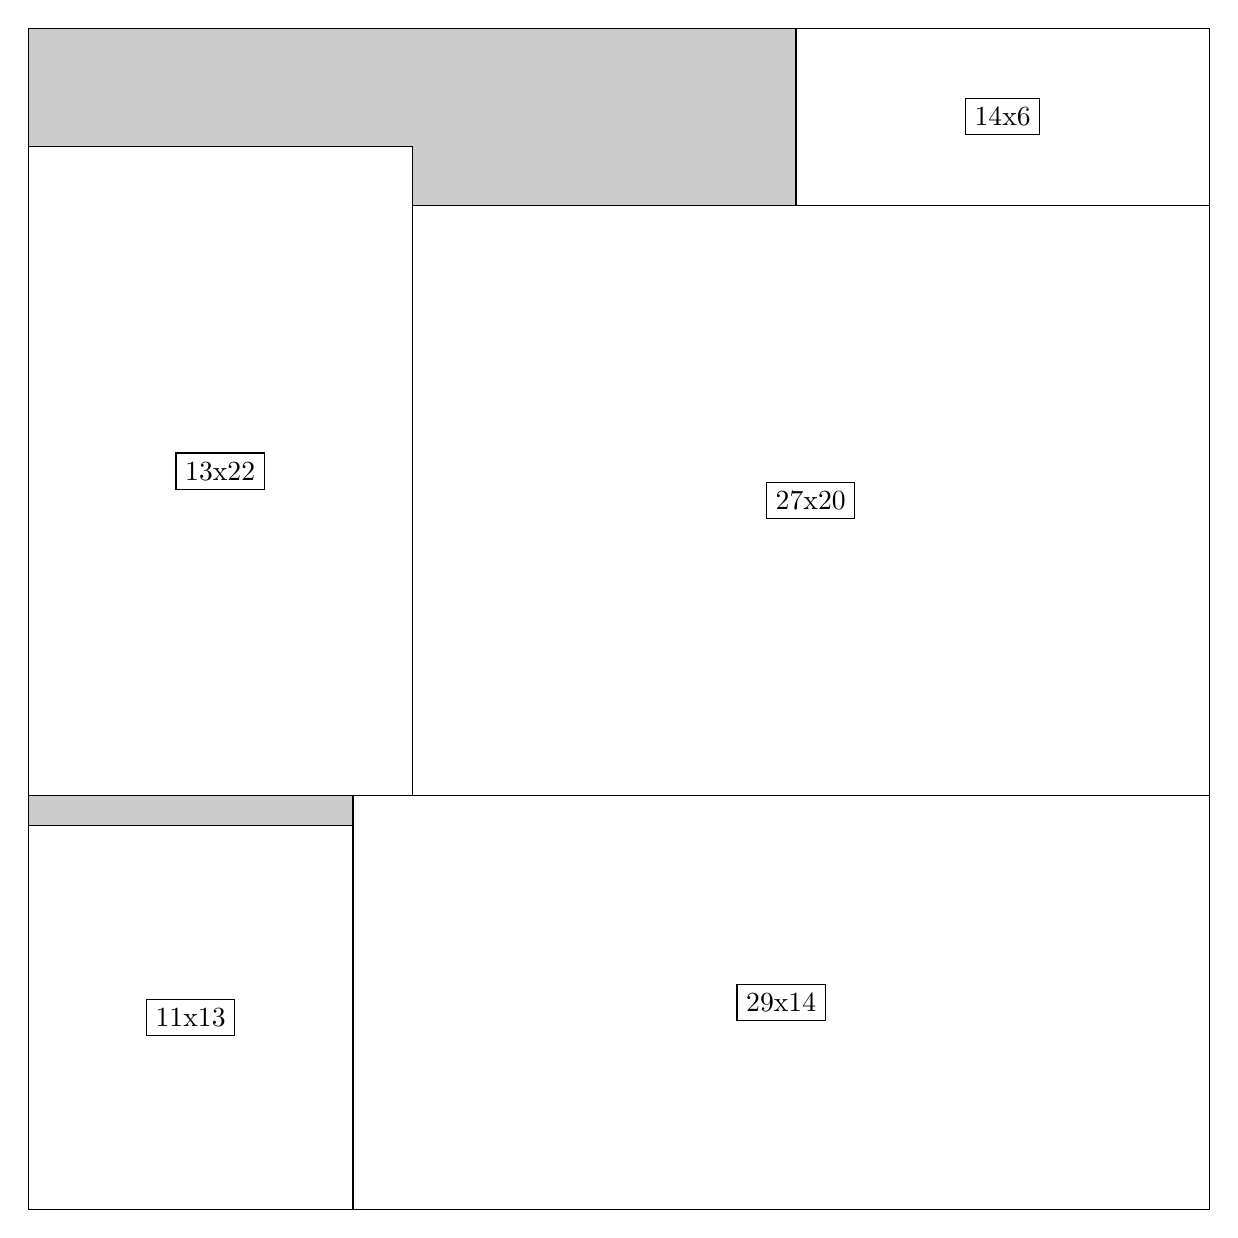
\begin{tikzpicture}[shorten >=1pt,scale=1.0,every node/.style={scale=1.0},->]
\tikzstyle{vertex}=[circle,fill=black!25,minimum size=14pt,inner sep=0pt]
\filldraw[fill=gray!40!white, draw=black] (0,0) rectangle (15.0,15.0);
\foreach \name/\x/\y/\w/\h in {29x14/4.125/0.0/10.875/5.25,11x13/0.0/0.0/4.125/4.875,27x20/4.875/5.25/10.125/7.5,14x6/9.75/12.75/5.25/2.25,13x22/0.0/5.25/4.875/8.25}
\filldraw[fill=white!40!white, draw=black] (\x,\y) rectangle node[draw] (\name) {\name} ++(\w,\h);
\end{tikzpicture}


w =29 , h =14 , x =11 , y =0 , v =406
\par
w =11 , h =13 , x =0 , y =0 , v =143
\par
w =27 , h =20 , x =13 , y =14 , v =540
\par
w =14 , h =6 , x =26 , y =34 , v =84
\par
w =13 , h =22 , x =0 , y =14 , v =286
\par
\newpage


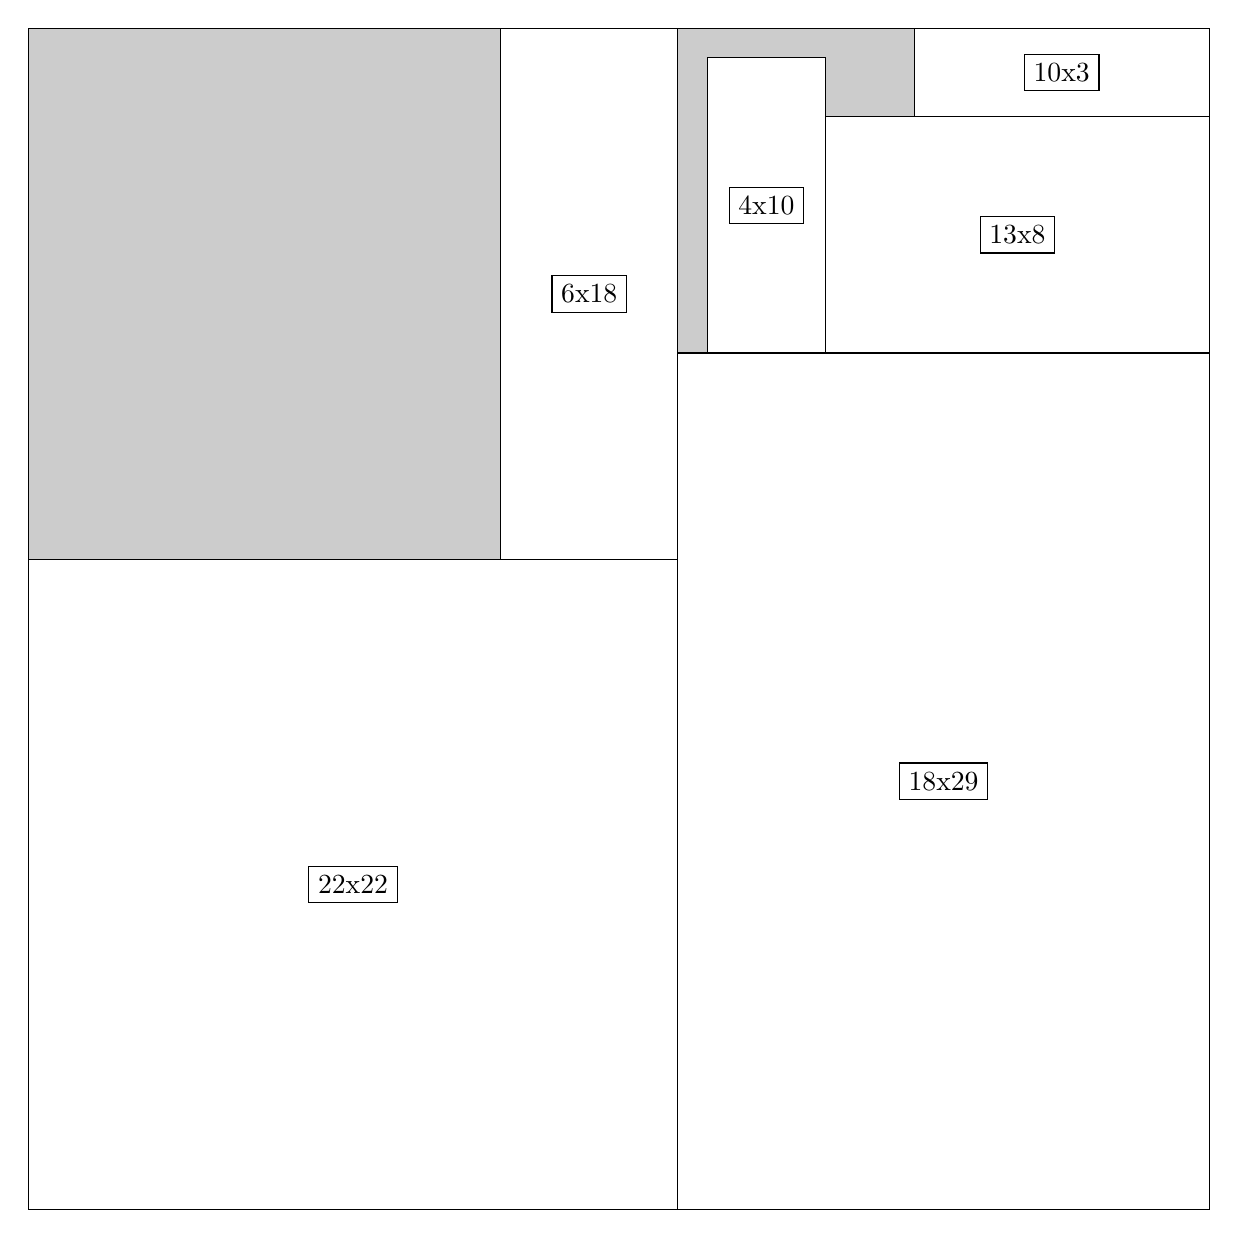
\begin{tikzpicture}[shorten >=1pt,scale=1.0,every node/.style={scale=1.0},->]
\tikzstyle{vertex}=[circle,fill=black!25,minimum size=14pt,inner sep=0pt]
\filldraw[fill=gray!40!white, draw=black] (0,0) rectangle (15.0,15.0);
\foreach \name/\x/\y/\w/\h in {18x29/8.25/0.0/6.75/10.875,13x8/10.125/10.875/4.875/3.0,10x3/11.25/13.875/3.75/1.125,4x10/8.625/10.875/1.5/3.75,22x22/0.0/0.0/8.25/8.25,6x18/6.0/8.25/2.25/6.75}
\filldraw[fill=white!40!white, draw=black] (\x,\y) rectangle node[draw] (\name) {\name} ++(\w,\h);
\end{tikzpicture}


w =18 , h =29 , x =22 , y =0 , v =522
\par
w =13 , h =8 , x =27 , y =29 , v =104
\par
w =10 , h =3 , x =30 , y =37 , v =30
\par
w =4 , h =10 , x =23 , y =29 , v =40
\par
w =22 , h =22 , x =0 , y =0 , v =484
\par
w =6 , h =18 , x =16 , y =22 , v =108
\par
\newpage


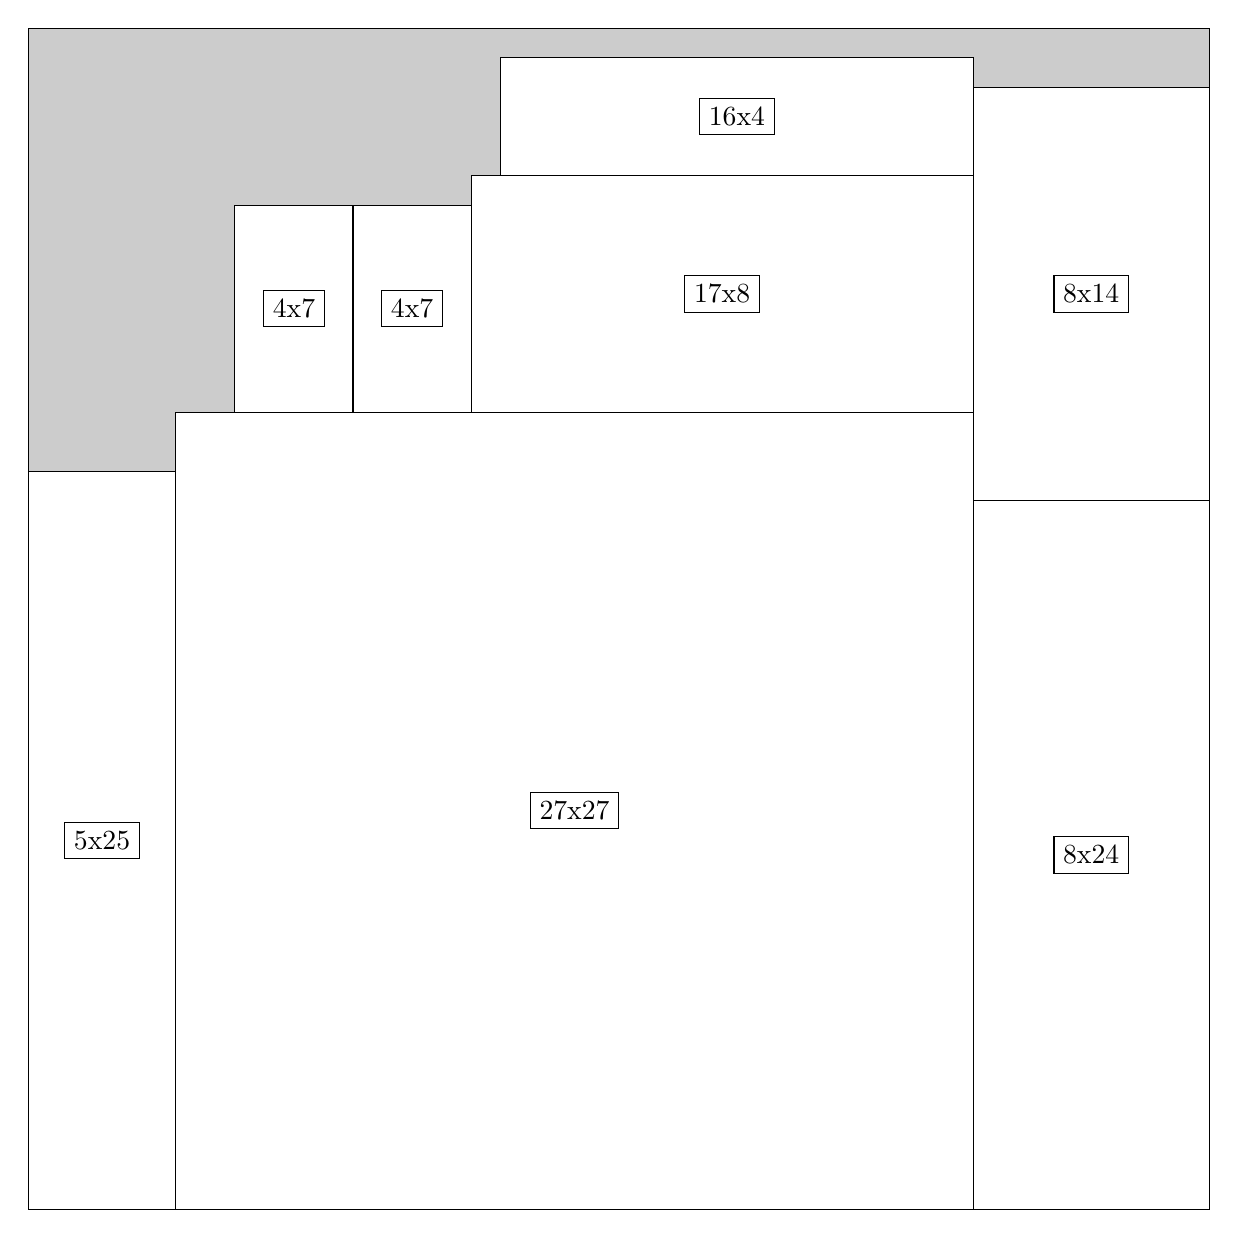
\begin{tikzpicture}[shorten >=1pt,scale=1.0,every node/.style={scale=1.0},->]
\tikzstyle{vertex}=[circle,fill=black!25,minimum size=14pt,inner sep=0pt]
\filldraw[fill=gray!40!white, draw=black] (0,0) rectangle (15.0,15.0);
\foreach \name/\x/\y/\w/\h in {8x24/12.0/0.0/3.0/9.0,8x14/12.0/9.0/3.0/5.25,27x27/1.875/0.0/10.125/10.125,17x8/5.625/10.125/6.375/3.0,4x7/4.125/10.125/1.5/2.625,4x7/2.625/10.125/1.5/2.625,16x4/6.0/13.125/6.0/1.5,5x25/0.0/0.0/1.875/9.375}
\filldraw[fill=white!40!white, draw=black] (\x,\y) rectangle node[draw] (\name) {\name} ++(\w,\h);
\end{tikzpicture}


w =8 , h =24 , x =32 , y =0 , v =192
\par
w =8 , h =14 , x =32 , y =24 , v =112
\par
w =27 , h =27 , x =5 , y =0 , v =729
\par
w =17 , h =8 , x =15 , y =27 , v =136
\par
w =4 , h =7 , x =11 , y =27 , v =28
\par
w =4 , h =7 , x =7 , y =27 , v =28
\par
w =16 , h =4 , x =16 , y =35 , v =64
\par
w =5 , h =25 , x =0 , y =0 , v =125
\par
\newpage


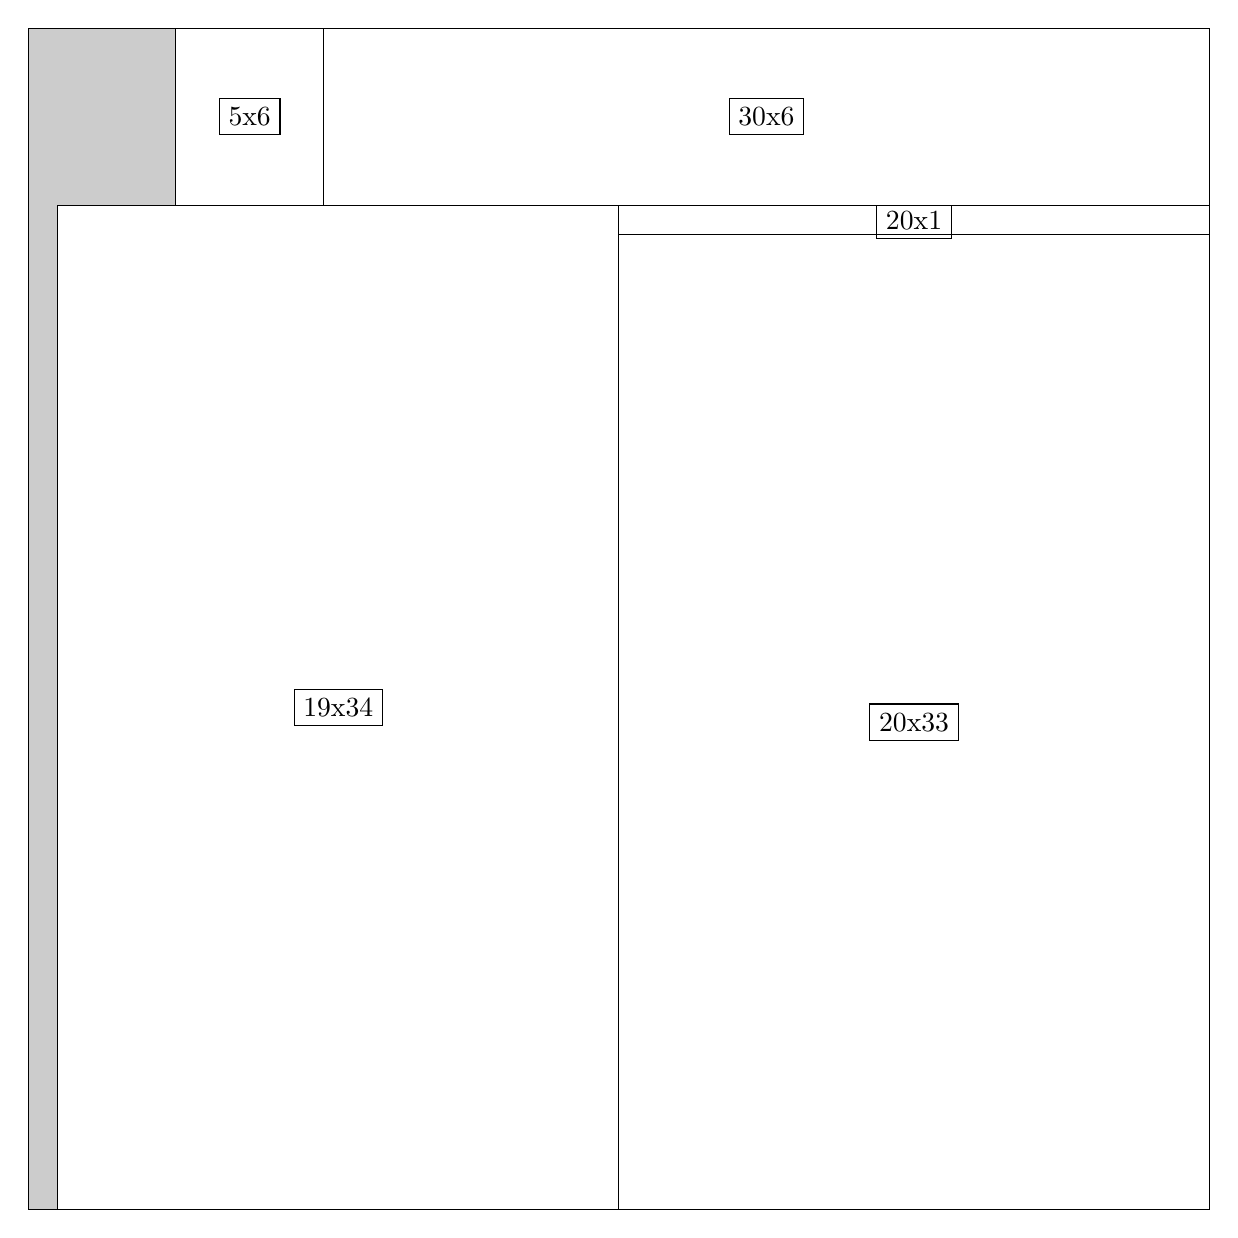
\begin{tikzpicture}[shorten >=1pt,scale=1.0,every node/.style={scale=1.0},->]
\tikzstyle{vertex}=[circle,fill=black!25,minimum size=14pt,inner sep=0pt]
\filldraw[fill=gray!40!white, draw=black] (0,0) rectangle (15.0,15.0);
\foreach \name/\x/\y/\w/\h in {20x33/7.5/0.0/7.5/12.375,20x1/7.5/12.375/7.5/0.375,19x34/0.375/0.0/7.125/12.75,30x6/3.75/12.75/11.25/2.25,5x6/1.875/12.75/1.875/2.25}
\filldraw[fill=white!40!white, draw=black] (\x,\y) rectangle node[draw] (\name) {\name} ++(\w,\h);
\end{tikzpicture}


w =20 , h =33 , x =20 , y =0 , v =660
\par
w =20 , h =1 , x =20 , y =33 , v =20
\par
w =19 , h =34 , x =1 , y =0 , v =646
\par
w =30 , h =6 , x =10 , y =34 , v =180
\par
w =5 , h =6 , x =5 , y =34 , v =30
\par
\newpage


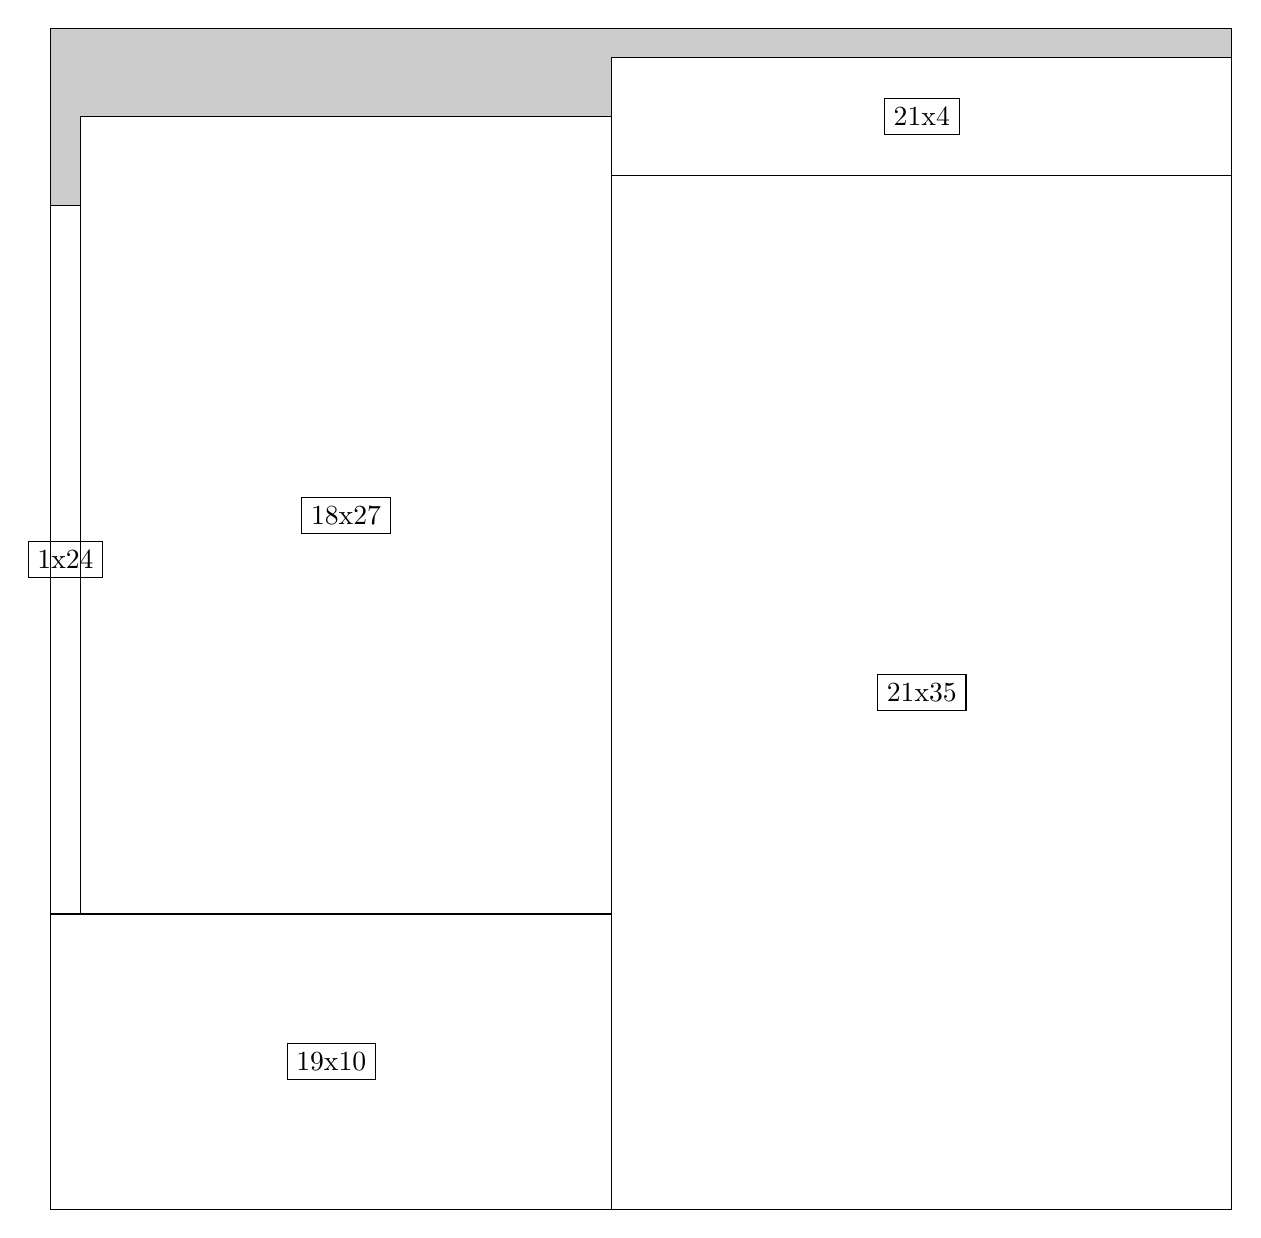
\begin{tikzpicture}[shorten >=1pt,scale=1.0,every node/.style={scale=1.0},->]
\tikzstyle{vertex}=[circle,fill=black!25,minimum size=14pt,inner sep=0pt]
\filldraw[fill=gray!40!white, draw=black] (0,0) rectangle (15.0,15.0);
\foreach \name/\x/\y/\w/\h in {21x35/7.125/0.0/7.875/13.125,21x4/7.125/13.125/7.875/1.5,19x10/0.0/0.0/7.125/3.75,18x27/0.375/3.75/6.75/10.125,1x24/0.0/3.75/0.375/9.0}
\filldraw[fill=white!40!white, draw=black] (\x,\y) rectangle node[draw] (\name) {\name} ++(\w,\h);
\end{tikzpicture}


w =21 , h =35 , x =19 , y =0 , v =735
\par
w =21 , h =4 , x =19 , y =35 , v =84
\par
w =19 , h =10 , x =0 , y =0 , v =190
\par
w =18 , h =27 , x =1 , y =10 , v =486
\par
w =1 , h =24 , x =0 , y =10 , v =24
\par
\newpage


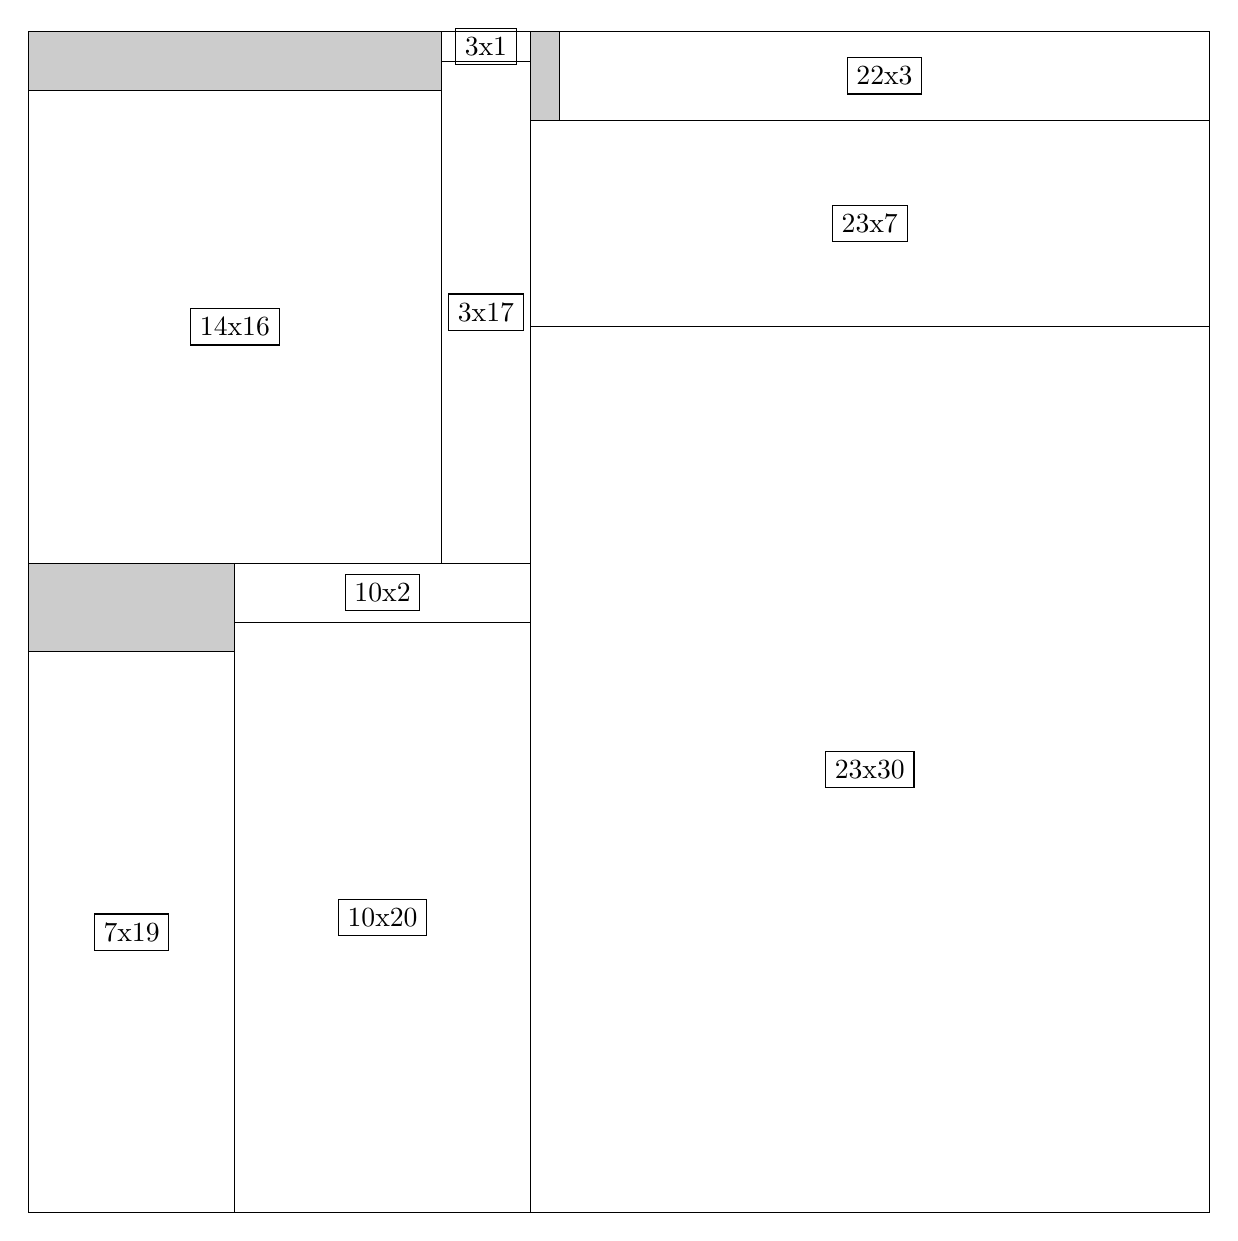
\begin{tikzpicture}[shorten >=1pt,scale=1.0,every node/.style={scale=1.0},->]
\tikzstyle{vertex}=[circle,fill=black!25,minimum size=14pt,inner sep=0pt]
\filldraw[fill=gray!40!white, draw=black] (0,0) rectangle (15.0,15.0);
\foreach \name/\x/\y/\w/\h in {23x30/6.375/0.0/8.625/11.25,23x7/6.375/11.25/8.625/2.625,22x3/6.75/13.875/8.25/1.125,10x20/2.625/0.0/3.75/7.5,10x2/2.625/7.5/3.75/0.75,7x19/0.0/0.0/2.625/7.125,3x17/5.25/8.25/1.125/6.375,3x1/5.25/14.625/1.125/0.375,14x16/0.0/8.25/5.25/6.0}
\filldraw[fill=white!40!white, draw=black] (\x,\y) rectangle node[draw] (\name) {\name} ++(\w,\h);
\end{tikzpicture}


w =23 , h =30 , x =17 , y =0 , v =690
\par
w =23 , h =7 , x =17 , y =30 , v =161
\par
w =22 , h =3 , x =18 , y =37 , v =66
\par
w =10 , h =20 , x =7 , y =0 , v =200
\par
w =10 , h =2 , x =7 , y =20 , v =20
\par
w =7 , h =19 , x =0 , y =0 , v =133
\par
w =3 , h =17 , x =14 , y =22 , v =51
\par
w =3 , h =1 , x =14 , y =39 , v =3
\par
w =14 , h =16 , x =0 , y =22 , v =224
\par
\newpage


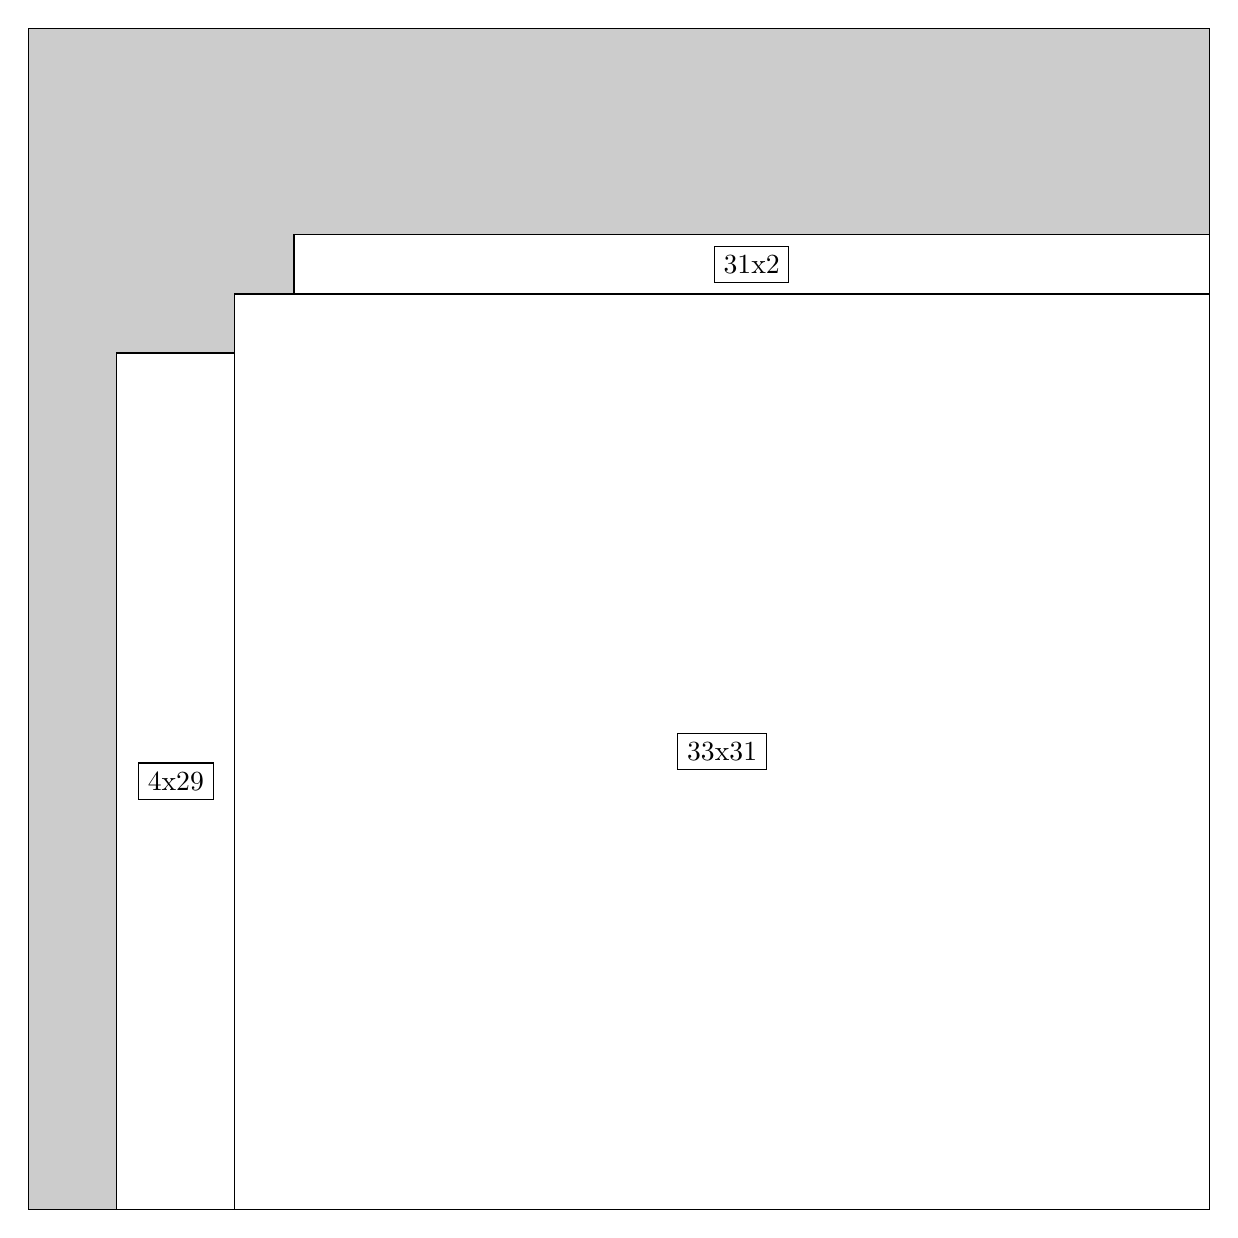
\begin{tikzpicture}[shorten >=1pt,scale=1.0,every node/.style={scale=1.0},->]
\tikzstyle{vertex}=[circle,fill=black!25,minimum size=14pt,inner sep=0pt]
\filldraw[fill=gray!40!white, draw=black] (0,0) rectangle (15.0,15.0);
\foreach \name/\x/\y/\w/\h in {33x31/2.625/0.0/12.375/11.625,31x2/3.375/11.625/11.625/0.75,4x29/1.125/0.0/1.5/10.875}
\filldraw[fill=white!40!white, draw=black] (\x,\y) rectangle node[draw] (\name) {\name} ++(\w,\h);
\end{tikzpicture}


w =33 , h =31 , x =7 , y =0 , v =1023
\par
w =31 , h =2 , x =9 , y =31 , v =62
\par
w =4 , h =29 , x =3 , y =0 , v =116
\par
\newpage


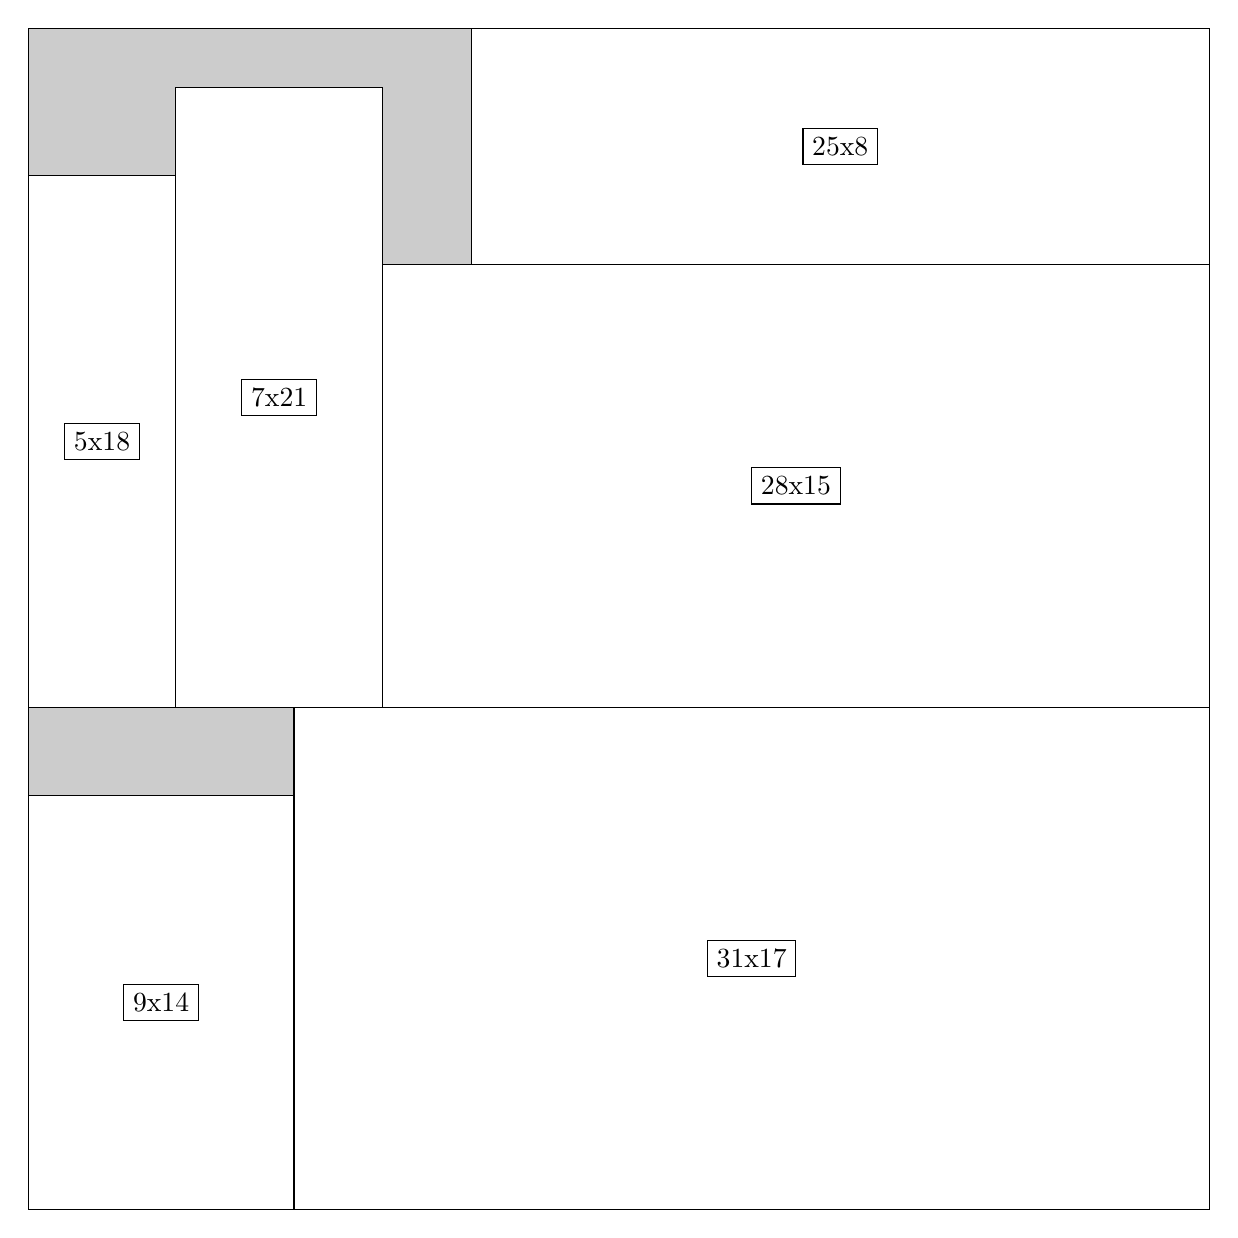
\begin{tikzpicture}[shorten >=1pt,scale=1.0,every node/.style={scale=1.0},->]
\tikzstyle{vertex}=[circle,fill=black!25,minimum size=14pt,inner sep=0pt]
\filldraw[fill=gray!40!white, draw=black] (0,0) rectangle (15.0,15.0);
\foreach \name/\x/\y/\w/\h in {31x17/3.375/0.0/11.625/6.375,9x14/0.0/0.0/3.375/5.25,28x15/4.5/6.375/10.5/5.625,25x8/5.625/12.0/9.375/3.0,7x21/1.875/6.375/2.625/7.875,5x18/0.0/6.375/1.875/6.75}
\filldraw[fill=white!40!white, draw=black] (\x,\y) rectangle node[draw] (\name) {\name} ++(\w,\h);
\end{tikzpicture}


w =31 , h =17 , x =9 , y =0 , v =527
\par
w =9 , h =14 , x =0 , y =0 , v =126
\par
w =28 , h =15 , x =12 , y =17 , v =420
\par
w =25 , h =8 , x =15 , y =32 , v =200
\par
w =7 , h =21 , x =5 , y =17 , v =147
\par
w =5 , h =18 , x =0 , y =17 , v =90
\par
\newpage


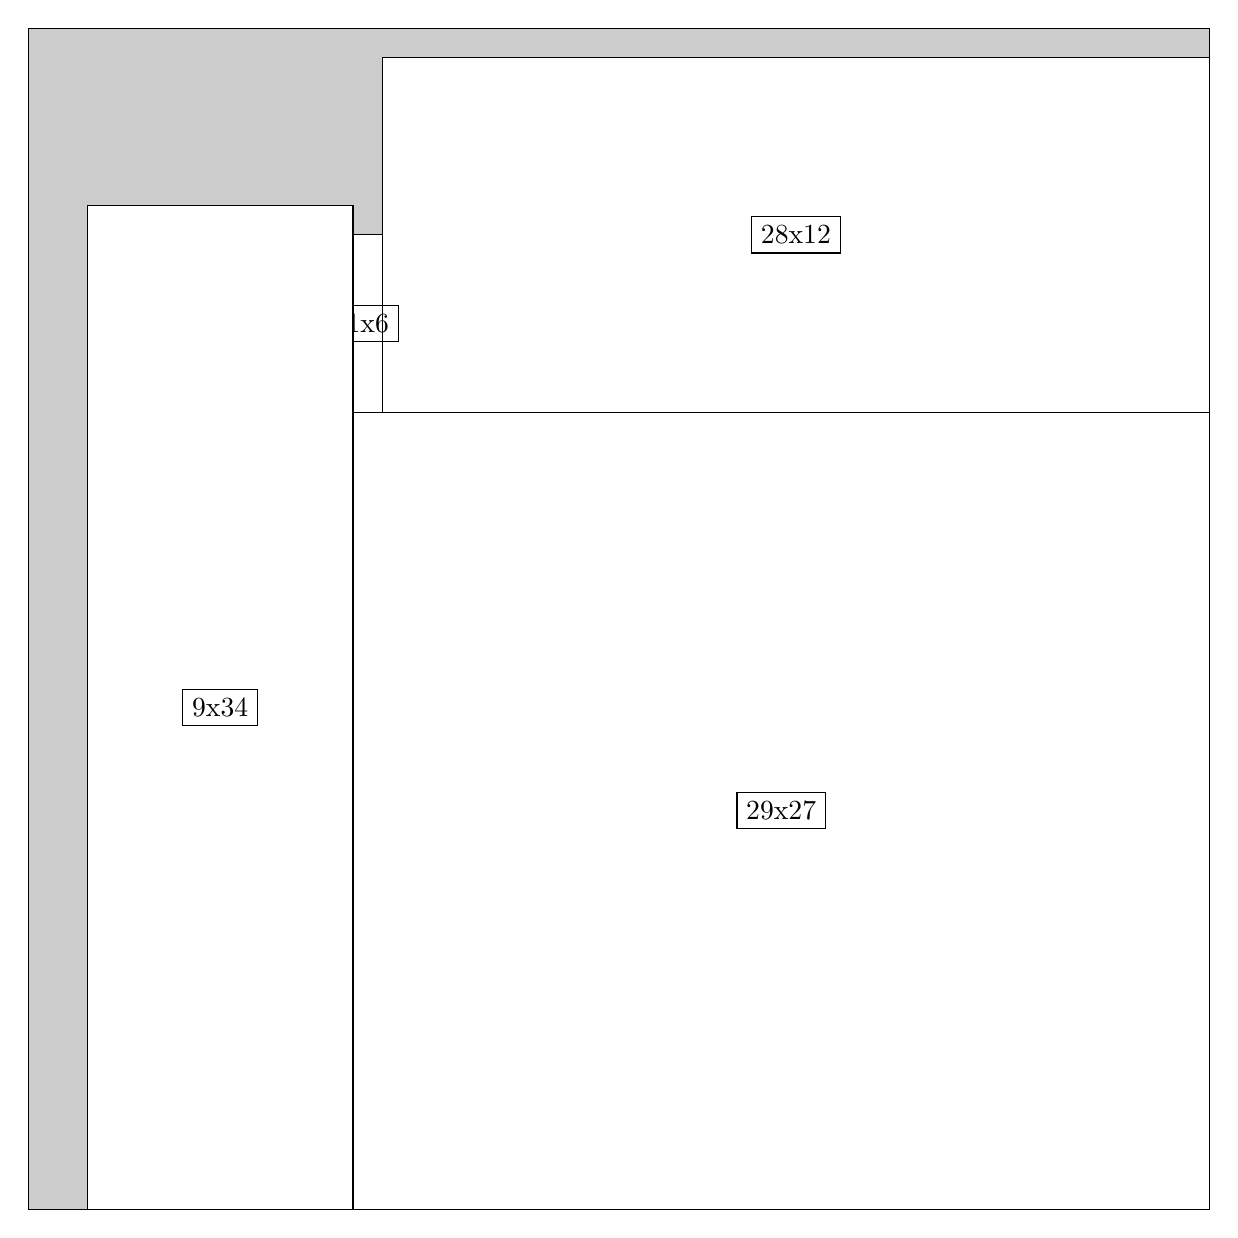
\begin{tikzpicture}[shorten >=1pt,scale=1.0,every node/.style={scale=1.0},->]
\tikzstyle{vertex}=[circle,fill=black!25,minimum size=14pt,inner sep=0pt]
\filldraw[fill=gray!40!white, draw=black] (0,0) rectangle (15.0,15.0);
\foreach \name/\x/\y/\w/\h in {29x27/4.125/0.0/10.875/10.125,28x12/4.5/10.125/10.5/4.5,1x6/4.125/10.125/0.375/2.25,9x34/0.75/0.0/3.375/12.75}
\filldraw[fill=white!40!white, draw=black] (\x,\y) rectangle node[draw] (\name) {\name} ++(\w,\h);
\end{tikzpicture}


w =29 , h =27 , x =11 , y =0 , v =783
\par
w =28 , h =12 , x =12 , y =27 , v =336
\par
w =1 , h =6 , x =11 , y =27 , v =6
\par
w =9 , h =34 , x =2 , y =0 , v =306
\par
\newpage


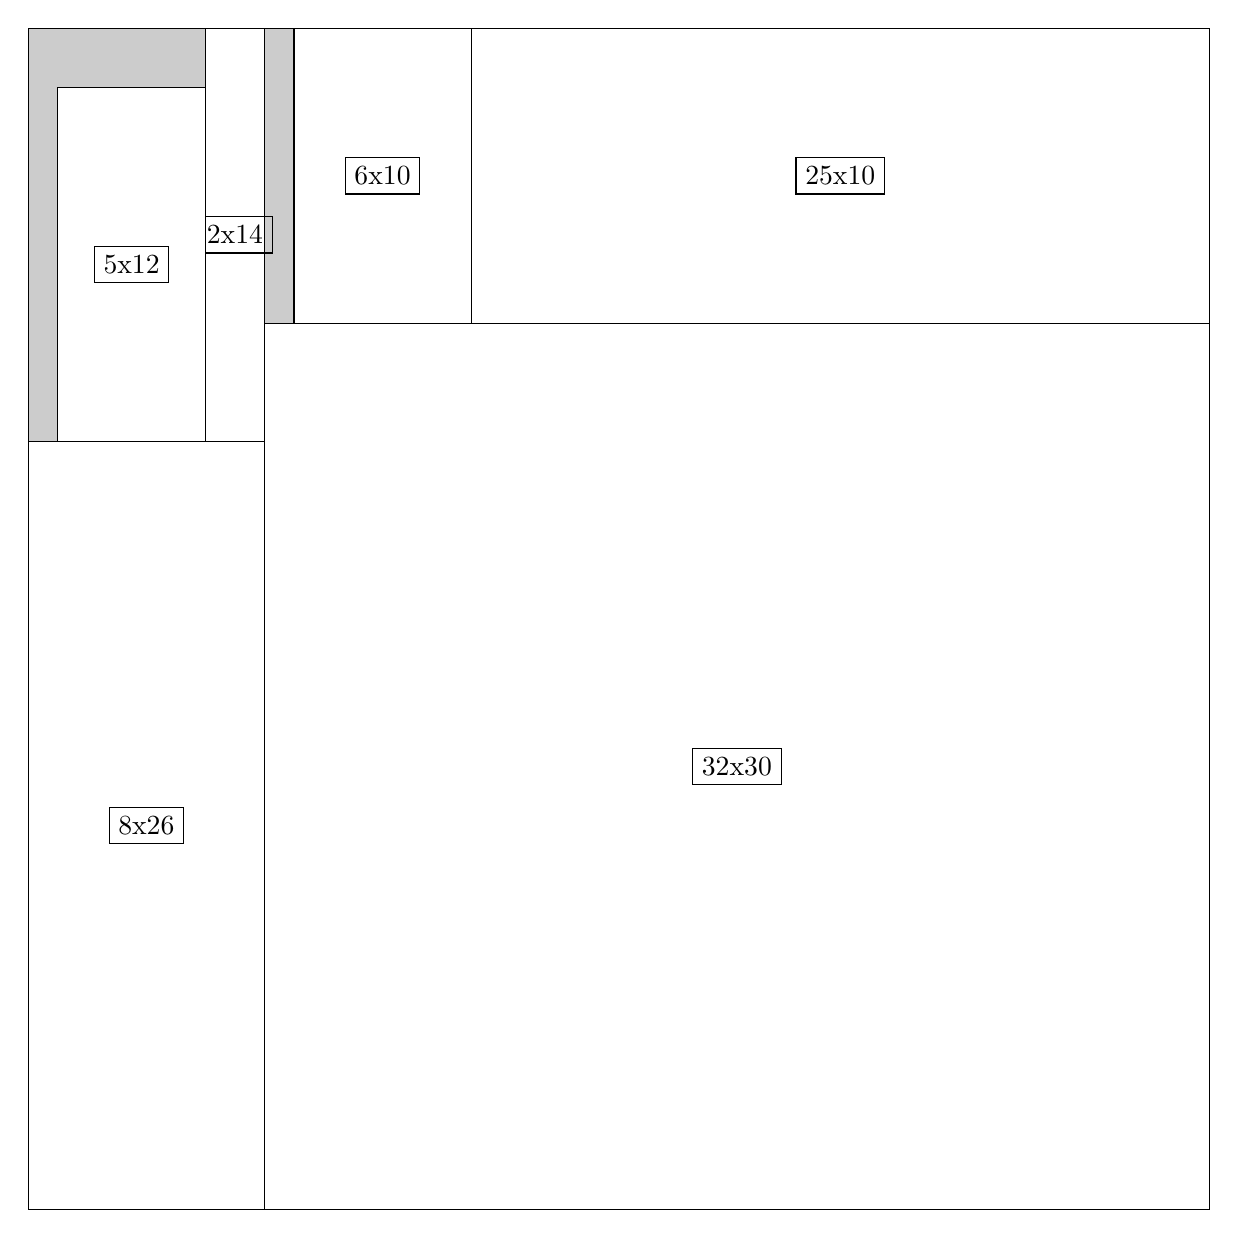
\begin{tikzpicture}[shorten >=1pt,scale=1.0,every node/.style={scale=1.0},->]
\tikzstyle{vertex}=[circle,fill=black!25,minimum size=14pt,inner sep=0pt]
\filldraw[fill=gray!40!white, draw=black] (0,0) rectangle (15.0,15.0);
\foreach \name/\x/\y/\w/\h in {32x30/3.0/0.0/12.0/11.25,25x10/5.625/11.25/9.375/3.75,6x10/3.375/11.25/2.25/3.75,8x26/0.0/0.0/3.0/9.75,2x14/2.25/9.75/0.75/5.25,5x12/0.375/9.75/1.875/4.5}
\filldraw[fill=white!40!white, draw=black] (\x,\y) rectangle node[draw] (\name) {\name} ++(\w,\h);
\end{tikzpicture}


w =32 , h =30 , x =8 , y =0 , v =960
\par
w =25 , h =10 , x =15 , y =30 , v =250
\par
w =6 , h =10 , x =9 , y =30 , v =60
\par
w =8 , h =26 , x =0 , y =0 , v =208
\par
w =2 , h =14 , x =6 , y =26 , v =28
\par
w =5 , h =12 , x =1 , y =26 , v =60
\par
\newpage


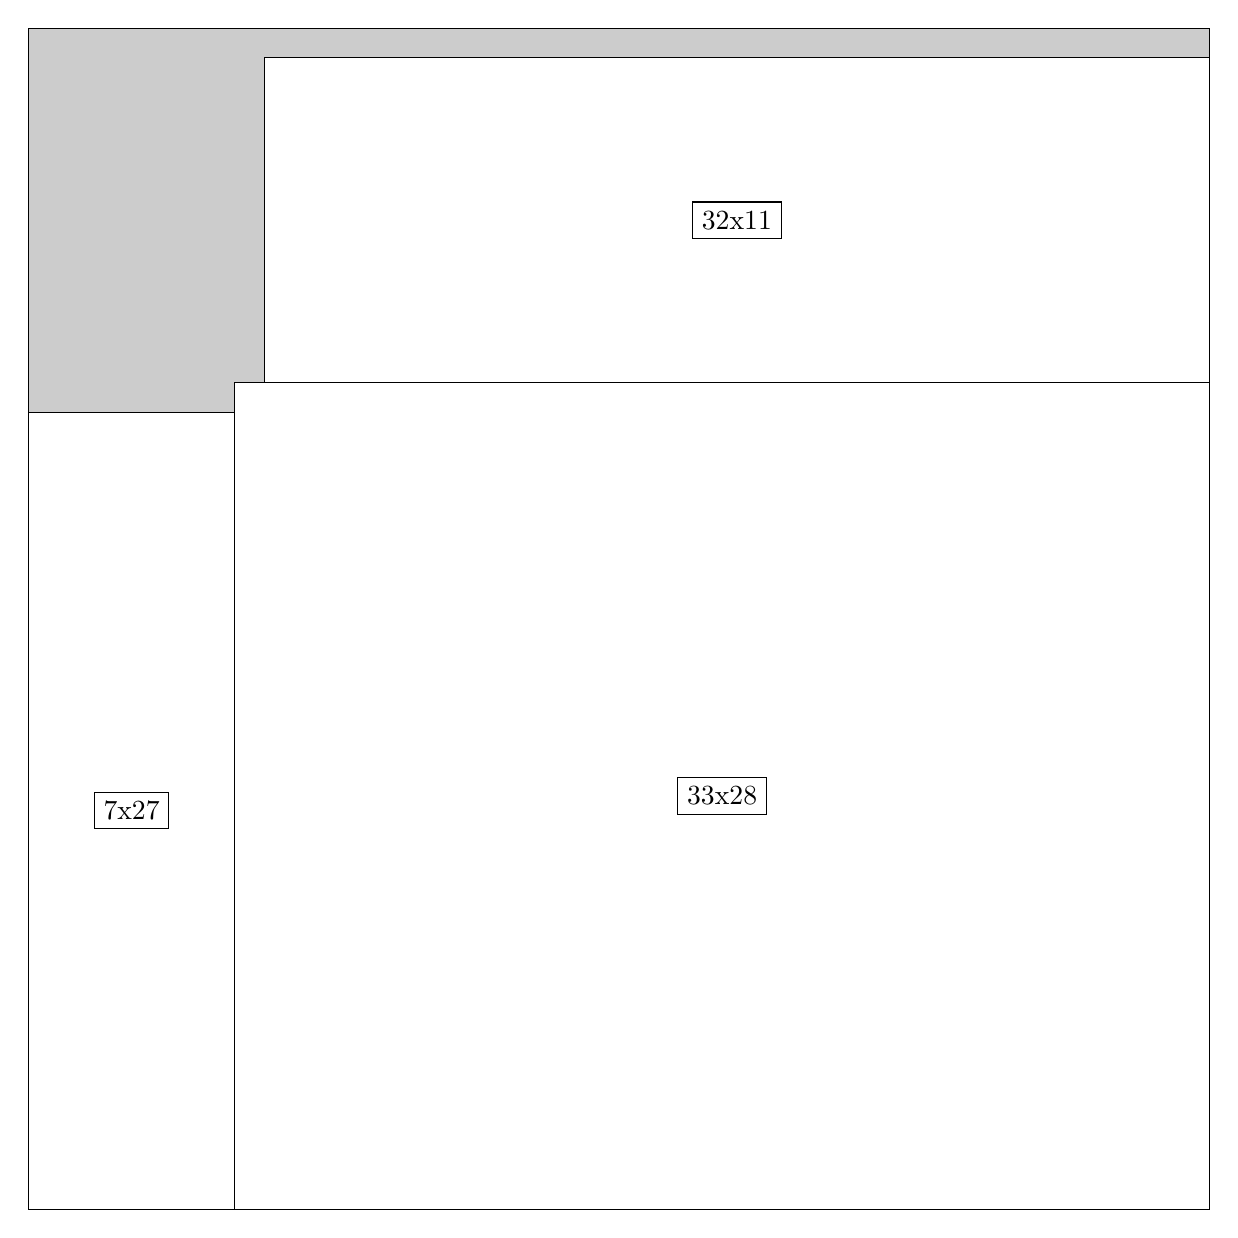
\begin{tikzpicture}[shorten >=1pt,scale=1.0,every node/.style={scale=1.0},->]
\tikzstyle{vertex}=[circle,fill=black!25,minimum size=14pt,inner sep=0pt]
\filldraw[fill=gray!40!white, draw=black] (0,0) rectangle (15.0,15.0);
\foreach \name/\x/\y/\w/\h in {33x28/2.625/0.0/12.375/10.5,7x27/0.0/0.0/2.625/10.125,32x11/3.0/10.5/12.0/4.125}
\filldraw[fill=white!40!white, draw=black] (\x,\y) rectangle node[draw] (\name) {\name} ++(\w,\h);
\end{tikzpicture}


w =33 , h =28 , x =7 , y =0 , v =924
\par
w =7 , h =27 , x =0 , y =0 , v =189
\par
w =32 , h =11 , x =8 , y =28 , v =352
\par
\newpage


\end{document}